% Created by tikzDevice version 0.12.6 on 2023-12-11 01:24:03
% !TEX encoding = UTF-8 Unicode
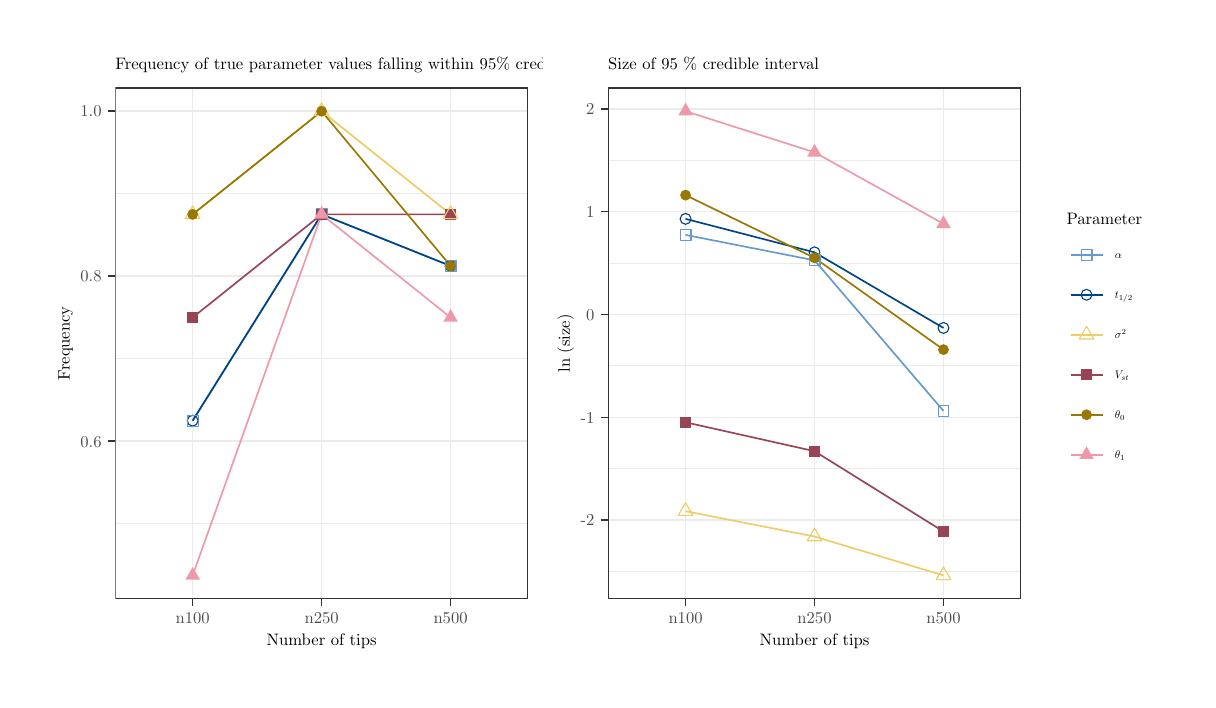
\begin{tikzpicture}[x=1pt,y=1pt]
\definecolor{fillColor}{RGB}{255,255,255}
\path[use as bounding box,fill=fillColor,fill opacity=0.00] (0,0) rectangle (419.17,235.60);
\begin{scope}
\path[clip] (  0.00,  0.00) rectangle (419.17,235.60);
\definecolor{drawColor}{RGB}{255,255,255}
\definecolor{fillColor}{RGB}{255,255,255}

\path[draw=drawColor,line width= 0.6pt,line join=round,line cap=round,fill=fillColor] (  0.00,  0.00) rectangle (419.17,235.60);
\end{scope}
\begin{scope}
\path[clip] (  5.50,  5.50) rectangle (186.28,230.10);
\definecolor{drawColor}{RGB}{255,255,255}
\definecolor{fillColor}{RGB}{255,255,255}

\path[draw=drawColor,line width= 0.6pt,line join=round,line cap=round,fill=fillColor] (  5.50,  5.50) rectangle (186.28,230.10);
\end{scope}
\begin{scope}
\path[clip] ( 31.66, 29.30) rectangle (180.78,213.80);
\definecolor{fillColor}{RGB}{255,255,255}

\path[fill=fillColor] ( 31.66, 29.30) rectangle (180.78,213.80);
\definecolor{drawColor}{gray}{0.92}

\path[draw=drawColor,line width= 0.3pt,line join=round] ( 31.66, 56.32) --
	(180.78, 56.32);

\path[draw=drawColor,line width= 0.3pt,line join=round] ( 31.66,115.96) --
	(180.78,115.96);

\path[draw=drawColor,line width= 0.3pt,line join=round] ( 31.66,175.60) --
	(180.78,175.60);

\path[draw=drawColor,line width= 0.6pt,line join=round] ( 31.66, 86.14) --
	(180.78, 86.14);

\path[draw=drawColor,line width= 0.6pt,line join=round] ( 31.66,145.78) --
	(180.78,145.78);

\path[draw=drawColor,line width= 0.6pt,line join=round] ( 31.66,205.41) --
	(180.78,205.41);

\path[draw=drawColor,line width= 0.6pt,line join=round] ( 59.62, 29.30) --
	( 59.62,213.80);

\path[draw=drawColor,line width= 0.6pt,line join=round] (106.22, 29.30) --
	(106.22,213.80);

\path[draw=drawColor,line width= 0.6pt,line join=round] (152.82, 29.30) --
	(152.82,213.80);
\definecolor{drawColor}{RGB}{102,153,204}

\path[draw=drawColor,line width= 0.6pt,line join=round] ( 59.62, 93.59) --
	(106.22,168.14) --
	(152.82,149.50);
\definecolor{drawColor}{RGB}{0,68,136}

\path[draw=drawColor,line width= 0.6pt,line join=round] ( 59.62, 93.59) --
	(106.22,168.14) --
	(152.82,149.50);
\definecolor{drawColor}{RGB}{238,204,102}

\path[draw=drawColor,line width= 0.6pt,line join=round] ( 59.62,168.14) --
	(106.22,205.41) --
	(152.82,168.14);
\definecolor{drawColor}{RGB}{153,68,85}

\path[draw=drawColor,line width= 0.6pt,line join=round] ( 59.62,130.87) --
	(106.22,168.14) --
	(152.82,168.14);
\definecolor{drawColor}{RGB}{153,119,0}

\path[draw=drawColor,line width= 0.6pt,line join=round] ( 59.62,168.14) --
	(106.22,205.41) --
	(152.82,149.50);
\definecolor{drawColor}{RGB}{238,153,170}

\path[draw=drawColor,line width= 0.6pt,line join=round] ( 59.62, 37.68) --
	(106.22,168.14) --
	(152.82,130.87);
\definecolor{drawColor}{RGB}{0,68,136}

\path[draw=drawColor,line width= 0.4pt,line join=round,line cap=round] ( 59.62, 93.59) circle (  1.96);
\definecolor{drawColor}{RGB}{102,153,204}

\path[draw=drawColor,line width= 0.4pt,line join=round,line cap=round] ( 57.66, 91.63) rectangle ( 61.58, 95.56);
\definecolor{fillColor}{RGB}{153,68,85}

\path[fill=fillColor] ( 57.66,128.91) --
	( 61.58,128.91) --
	( 61.58,132.83) --
	( 57.66,132.83) --
	cycle;
\definecolor{drawColor}{RGB}{238,204,102}

\path[draw=drawColor,line width= 0.4pt,line join=round,line cap=round] ( 59.62,171.19) --
	( 62.27,166.62) --
	( 56.98,166.62) --
	cycle;
\definecolor{fillColor}{RGB}{153,119,0}

\path[fill=fillColor] ( 59.62,168.14) circle (  1.96);
\definecolor{fillColor}{RGB}{238,153,170}

\path[fill=fillColor] ( 59.62, 40.74) --
	( 62.27, 36.16) --
	( 56.98, 36.16) --
	cycle;
\definecolor{drawColor}{RGB}{0,68,136}

\path[draw=drawColor,line width= 0.4pt,line join=round,line cap=round] (106.22,168.14) circle (  1.96);
\definecolor{drawColor}{RGB}{102,153,204}

\path[draw=drawColor,line width= 0.4pt,line join=round,line cap=round] (104.26,166.18) rectangle (108.18,170.10);
\definecolor{fillColor}{RGB}{153,68,85}

\path[fill=fillColor] (104.26,166.18) --
	(108.18,166.18) --
	(108.18,170.10) --
	(104.26,170.10) --
	cycle;
\definecolor{drawColor}{RGB}{238,204,102}

\path[draw=drawColor,line width= 0.4pt,line join=round,line cap=round] (106.22,208.47) --
	(108.86,203.89) --
	(103.58,203.89) --
	cycle;
\definecolor{fillColor}{RGB}{153,119,0}

\path[fill=fillColor] (106.22,205.41) circle (  1.96);
\definecolor{fillColor}{RGB}{238,153,170}

\path[fill=fillColor] (106.22,171.19) --
	(108.86,166.62) --
	(103.58,166.62) --
	cycle;
\definecolor{drawColor}{RGB}{0,68,136}

\path[draw=drawColor,line width= 0.4pt,line join=round,line cap=round] (152.82,149.50) circle (  1.96);
\definecolor{drawColor}{RGB}{102,153,204}

\path[draw=drawColor,line width= 0.4pt,line join=round,line cap=round] (150.86,147.54) rectangle (154.78,151.47);
\definecolor{fillColor}{RGB}{153,68,85}

\path[fill=fillColor] (150.86,166.18) --
	(154.78,166.18) --
	(154.78,170.10) --
	(150.86,170.10) --
	cycle;
\definecolor{drawColor}{RGB}{238,204,102}

\path[draw=drawColor,line width= 0.4pt,line join=round,line cap=round] (152.82,171.19) --
	(155.46,166.62) --
	(150.18,166.62) --
	cycle;
\definecolor{fillColor}{RGB}{153,119,0}

\path[fill=fillColor] (152.82,149.50) circle (  1.96);
\definecolor{fillColor}{RGB}{238,153,170}

\path[fill=fillColor] (152.82,133.92) --
	(155.46,129.34) --
	(150.18,129.34) --
	cycle;
\definecolor{drawColor}{gray}{0.20}

\path[draw=drawColor,line width= 0.6pt,line join=round,line cap=round] ( 31.66, 29.30) rectangle (180.78,213.80);
\end{scope}
\begin{scope}
\path[clip] (  0.00,  0.00) rectangle (419.17,235.60);
\definecolor{drawColor}{gray}{0.30}

\node[text=drawColor,anchor=base east,inner sep=0pt, outer sep=0pt, scale=  0.60] at ( 26.71, 84.07) {0.6};

\node[text=drawColor,anchor=base east,inner sep=0pt, outer sep=0pt, scale=  0.60] at ( 26.71,143.71) {0.8};

\node[text=drawColor,anchor=base east,inner sep=0pt, outer sep=0pt, scale=  0.60] at ( 26.71,203.35) {1.0};
\end{scope}
\begin{scope}
\path[clip] (  0.00,  0.00) rectangle (419.17,235.60);
\definecolor{drawColor}{gray}{0.20}

\path[draw=drawColor,line width= 0.6pt,line join=round] ( 28.91, 86.14) --
	( 31.66, 86.14);

\path[draw=drawColor,line width= 0.6pt,line join=round] ( 28.91,145.78) --
	( 31.66,145.78);

\path[draw=drawColor,line width= 0.6pt,line join=round] ( 28.91,205.41) --
	( 31.66,205.41);
\end{scope}
\begin{scope}
\path[clip] (  0.00,  0.00) rectangle (419.17,235.60);
\definecolor{drawColor}{gray}{0.20}

\path[draw=drawColor,line width= 0.6pt,line join=round] ( 59.62, 26.55) --
	( 59.62, 29.30);

\path[draw=drawColor,line width= 0.6pt,line join=round] (106.22, 26.55) --
	(106.22, 29.30);

\path[draw=drawColor,line width= 0.6pt,line join=round] (152.82, 26.55) --
	(152.82, 29.30);
\end{scope}
\begin{scope}
\path[clip] (  0.00,  0.00) rectangle (419.17,235.60);
\definecolor{drawColor}{gray}{0.30}

\node[text=drawColor,anchor=base,inner sep=0pt, outer sep=0pt, scale=  0.60] at ( 59.62, 20.22) {n100};

\node[text=drawColor,anchor=base,inner sep=0pt, outer sep=0pt, scale=  0.60] at (106.22, 20.22) {n250};

\node[text=drawColor,anchor=base,inner sep=0pt, outer sep=0pt, scale=  0.60] at (152.82, 20.22) {n500};
\end{scope}
\begin{scope}
\path[clip] (  0.00,  0.00) rectangle (419.17,235.60);
\definecolor{drawColor}{RGB}{0,0,0}

\node[text=drawColor,anchor=base,inner sep=0pt, outer sep=0pt, scale=  0.60] at (106.22, 12.17) {Number of tips};
\end{scope}
\begin{scope}
\path[clip] (  0.00,  0.00) rectangle (419.17,235.60);
\definecolor{drawColor}{RGB}{0,0,0}

\node[text=drawColor,rotate= 90.00,anchor=base,inner sep=0pt, outer sep=0pt, scale=  0.60] at ( 15.13,121.55) {Frequency};
\end{scope}
\begin{scope}
\path[clip] (  0.00,  0.00) rectangle (419.17,235.60);
\definecolor{drawColor}{RGB}{0,0,0}

\node[text=drawColor,anchor=base west,inner sep=0pt, outer sep=0pt, scale=  0.60] at ( 31.66,220.47) {Frequency of true parameter values falling within  $\newline 95\%$ credible interval};
\end{scope}
\begin{scope}
\path[clip] (186.28,  5.50) rectangle (413.67,230.10);
\definecolor{drawColor}{RGB}{255,255,255}
\definecolor{fillColor}{RGB}{255,255,255}

\path[draw=drawColor,line width= 0.6pt,line join=round,line cap=round,fill=fillColor] (186.28,  5.50) rectangle (413.67,230.10);
\end{scope}
\begin{scope}
\path[clip] (209.78, 29.30) rectangle (358.89,213.80);
\definecolor{fillColor}{RGB}{255,255,255}

\path[fill=fillColor] (209.78, 29.30) rectangle (358.89,213.80);
\definecolor{drawColor}{gray}{0.92}

\path[draw=drawColor,line width= 0.3pt,line join=round] (209.78, 39.04) --
	(358.89, 39.04);

\path[draw=drawColor,line width= 0.3pt,line join=round] (209.78, 76.21) --
	(358.89, 76.21);

\path[draw=drawColor,line width= 0.3pt,line join=round] (209.78,113.38) --
	(358.89,113.38);

\path[draw=drawColor,line width= 0.3pt,line join=round] (209.78,150.54) --
	(358.89,150.54);

\path[draw=drawColor,line width= 0.3pt,line join=round] (209.78,187.71) --
	(358.89,187.71);

\path[draw=drawColor,line width= 0.6pt,line join=round] (209.78, 57.63) --
	(358.89, 57.63);

\path[draw=drawColor,line width= 0.6pt,line join=round] (209.78, 94.79) --
	(358.89, 94.79);

\path[draw=drawColor,line width= 0.6pt,line join=round] (209.78,131.96) --
	(358.89,131.96);

\path[draw=drawColor,line width= 0.6pt,line join=round] (209.78,169.13) --
	(358.89,169.13);

\path[draw=drawColor,line width= 0.6pt,line join=round] (209.78,206.29) --
	(358.89,206.29);

\path[draw=drawColor,line width= 0.6pt,line join=round] (237.73, 29.30) --
	(237.73,213.80);

\path[draw=drawColor,line width= 0.6pt,line join=round] (284.33, 29.30) --
	(284.33,213.80);

\path[draw=drawColor,line width= 0.6pt,line join=round] (330.93, 29.30) --
	(330.93,213.80);
\definecolor{drawColor}{RGB}{102,153,204}

\path[draw=drawColor,line width= 0.6pt,line join=round] (237.73,160.72) --
	(284.33,151.52) --
	(330.93, 97.10);
\definecolor{drawColor}{RGB}{0,68,136}

\path[draw=drawColor,line width= 0.6pt,line join=round] (237.73,166.51) --
	(284.33,154.42) --
	(330.93,127.09);
\definecolor{drawColor}{RGB}{238,204,102}

\path[draw=drawColor,line width= 0.6pt,line join=round] (237.73, 60.87) --
	(284.33, 51.72) --
	(330.93, 37.68);
\definecolor{drawColor}{RGB}{153,68,85}

\path[draw=drawColor,line width= 0.6pt,line join=round] (237.73, 93.00) --
	(284.33, 82.56) --
	(330.93, 53.53);
\definecolor{drawColor}{RGB}{153,119,0}

\path[draw=drawColor,line width= 0.6pt,line join=round] (237.73,175.08) --
	(284.33,152.42) --
	(330.93,119.26);
\definecolor{drawColor}{RGB}{238,153,170}

\path[draw=drawColor,line width= 0.6pt,line join=round] (237.73,205.41) --
	(284.33,190.56) --
	(330.93,164.73);
\definecolor{drawColor}{RGB}{0,68,136}

\path[draw=drawColor,line width= 0.4pt,line join=round,line cap=round] (237.73,166.51) circle (  1.96);
\definecolor{drawColor}{RGB}{102,153,204}

\path[draw=drawColor,line width= 0.4pt,line join=round,line cap=round] (235.77,158.76) rectangle (239.70,162.68);
\definecolor{fillColor}{RGB}{153,68,85}

\path[fill=fillColor] (235.77, 91.04) --
	(239.70, 91.04) --
	(239.70, 94.97) --
	(235.77, 94.97) --
	cycle;
\definecolor{drawColor}{RGB}{238,204,102}

\path[draw=drawColor,line width= 0.4pt,line join=round,line cap=round] (237.73, 63.93) --
	(240.38, 59.35) --
	(235.09, 59.35) --
	cycle;
\definecolor{fillColor}{RGB}{153,119,0}

\path[fill=fillColor] (237.73,175.08) circle (  1.96);
\definecolor{fillColor}{RGB}{238,153,170}

\path[fill=fillColor] (237.73,208.47) --
	(240.38,203.89) --
	(235.09,203.89) --
	cycle;
\definecolor{drawColor}{RGB}{0,68,136}

\path[draw=drawColor,line width= 0.4pt,line join=round,line cap=round] (284.33,154.42) circle (  1.96);
\definecolor{drawColor}{RGB}{102,153,204}

\path[draw=drawColor,line width= 0.4pt,line join=round,line cap=round] (282.37,149.56) rectangle (286.29,153.49);
\definecolor{fillColor}{RGB}{153,68,85}

\path[fill=fillColor] (282.37, 80.60) --
	(286.29, 80.60) --
	(286.29, 84.52) --
	(282.37, 84.52) --
	cycle;
\definecolor{drawColor}{RGB}{238,204,102}

\path[draw=drawColor,line width= 0.4pt,line join=round,line cap=round] (284.33, 54.77) --
	(286.97, 50.19) --
	(281.69, 50.19) --
	cycle;
\definecolor{fillColor}{RGB}{153,119,0}

\path[fill=fillColor] (284.33,152.42) circle (  1.96);
\definecolor{fillColor}{RGB}{238,153,170}

\path[fill=fillColor] (284.33,193.61) --
	(286.97,189.04) --
	(281.69,189.04) --
	cycle;
\definecolor{drawColor}{RGB}{0,68,136}

\path[draw=drawColor,line width= 0.4pt,line join=round,line cap=round] (330.93,127.09) circle (  1.96);
\definecolor{drawColor}{RGB}{102,153,204}

\path[draw=drawColor,line width= 0.4pt,line join=round,line cap=round] (328.97, 95.14) rectangle (332.89, 99.06);
\definecolor{fillColor}{RGB}{153,68,85}

\path[fill=fillColor] (328.97, 51.57) --
	(332.89, 51.57) --
	(332.89, 55.49) --
	(328.97, 55.49) --
	cycle;
\definecolor{drawColor}{RGB}{238,204,102}

\path[draw=drawColor,line width= 0.4pt,line join=round,line cap=round] (330.93, 40.74) --
	(333.57, 36.16) --
	(328.29, 36.16) --
	cycle;
\definecolor{fillColor}{RGB}{153,119,0}

\path[fill=fillColor] (330.93,119.26) circle (  1.96);
\definecolor{fillColor}{RGB}{238,153,170}

\path[fill=fillColor] (330.93,167.78) --
	(333.57,163.20) --
	(328.29,163.20) --
	cycle;
\definecolor{drawColor}{gray}{0.20}

\path[draw=drawColor,line width= 0.6pt,line join=round,line cap=round] (209.78, 29.30) rectangle (358.89,213.80);
\end{scope}
\begin{scope}
\path[clip] (  0.00,  0.00) rectangle (419.17,235.60);
\definecolor{drawColor}{gray}{0.30}

\node[text=drawColor,anchor=base east,inner sep=0pt, outer sep=0pt, scale=  0.60] at (204.83, 55.56) {-2};

\node[text=drawColor,anchor=base east,inner sep=0pt, outer sep=0pt, scale=  0.60] at (204.83, 92.73) {-1};

\node[text=drawColor,anchor=base east,inner sep=0pt, outer sep=0pt, scale=  0.60] at (204.83,129.89) {0};

\node[text=drawColor,anchor=base east,inner sep=0pt, outer sep=0pt, scale=  0.60] at (204.83,167.06) {1};

\node[text=drawColor,anchor=base east,inner sep=0pt, outer sep=0pt, scale=  0.60] at (204.83,204.23) {2};
\end{scope}
\begin{scope}
\path[clip] (  0.00,  0.00) rectangle (419.17,235.60);
\definecolor{drawColor}{gray}{0.20}

\path[draw=drawColor,line width= 0.6pt,line join=round] (207.03, 57.63) --
	(209.78, 57.63);

\path[draw=drawColor,line width= 0.6pt,line join=round] (207.03, 94.79) --
	(209.78, 94.79);

\path[draw=drawColor,line width= 0.6pt,line join=round] (207.03,131.96) --
	(209.78,131.96);

\path[draw=drawColor,line width= 0.6pt,line join=round] (207.03,169.13) --
	(209.78,169.13);

\path[draw=drawColor,line width= 0.6pt,line join=round] (207.03,206.29) --
	(209.78,206.29);
\end{scope}
\begin{scope}
\path[clip] (  0.00,  0.00) rectangle (419.17,235.60);
\definecolor{drawColor}{gray}{0.20}

\path[draw=drawColor,line width= 0.6pt,line join=round] (237.73, 26.55) --
	(237.73, 29.30);

\path[draw=drawColor,line width= 0.6pt,line join=round] (284.33, 26.55) --
	(284.33, 29.30);

\path[draw=drawColor,line width= 0.6pt,line join=round] (330.93, 26.55) --
	(330.93, 29.30);
\end{scope}
\begin{scope}
\path[clip] (  0.00,  0.00) rectangle (419.17,235.60);
\definecolor{drawColor}{gray}{0.30}

\node[text=drawColor,anchor=base,inner sep=0pt, outer sep=0pt, scale=  0.60] at (237.73, 20.22) {n100};

\node[text=drawColor,anchor=base,inner sep=0pt, outer sep=0pt, scale=  0.60] at (284.33, 20.22) {n250};

\node[text=drawColor,anchor=base,inner sep=0pt, outer sep=0pt, scale=  0.60] at (330.93, 20.22) {n500};
\end{scope}
\begin{scope}
\path[clip] (  0.00,  0.00) rectangle (419.17,235.60);
\definecolor{drawColor}{RGB}{0,0,0}

\node[text=drawColor,anchor=base,inner sep=0pt, outer sep=0pt, scale=  0.60] at (284.33, 12.17) {Number of tips};
\end{scope}
\begin{scope}
\path[clip] (  0.00,  0.00) rectangle (419.17,235.60);
\definecolor{drawColor}{RGB}{0,0,0}

\node[text=drawColor,rotate= 90.00,anchor=base,inner sep=0pt, outer sep=0pt, scale=  0.60] at (195.91,121.55) {$\ln$ (size)};
\end{scope}
\begin{scope}
\path[clip] (  0.00,  0.00) rectangle (419.17,235.60);
\definecolor{fillColor}{RGB}{255,255,255}

\path[fill=fillColor] (369.89, 68.54) rectangle (408.17,174.56);
\end{scope}
\begin{scope}
\path[clip] (  0.00,  0.00) rectangle (419.17,235.60);
\definecolor{drawColor}{RGB}{0,0,0}

\node[text=drawColor,anchor=base west,inner sep=0pt, outer sep=0pt, scale=  0.60] at (375.39,164.35) {Parameter};
\end{scope}
\begin{scope}
\path[clip] (  0.00,  0.00) rectangle (419.17,235.60);
\definecolor{fillColor}{RGB}{255,255,255}

\path[fill=fillColor] (375.39,146.31) rectangle (389.84,160.76);
\end{scope}
\begin{scope}
\path[clip] (  0.00,  0.00) rectangle (419.17,235.60);
\definecolor{drawColor}{RGB}{102,153,204}

\path[draw=drawColor,line width= 0.6pt,line join=round] (376.83,153.54) -- (388.40,153.54);
\end{scope}
\begin{scope}
\path[clip] (  0.00,  0.00) rectangle (419.17,235.60);
\definecolor{drawColor}{RGB}{102,153,204}

\path[draw=drawColor,line width= 0.4pt,line join=round,line cap=round] (380.65,151.57) rectangle (384.58,155.50);
\end{scope}
\begin{scope}
\path[clip] (  0.00,  0.00) rectangle (419.17,235.60);
\definecolor{fillColor}{RGB}{255,255,255}

\path[fill=fillColor] (375.39,131.85) rectangle (389.84,146.31);
\end{scope}
\begin{scope}
\path[clip] (  0.00,  0.00) rectangle (419.17,235.60);
\definecolor{drawColor}{RGB}{0,68,136}

\path[draw=drawColor,line width= 0.6pt,line join=round] (376.83,139.08) -- (388.40,139.08);
\end{scope}
\begin{scope}
\path[clip] (  0.00,  0.00) rectangle (419.17,235.60);
\definecolor{drawColor}{RGB}{0,68,136}

\path[draw=drawColor,line width= 0.4pt,line join=round,line cap=round] (382.62,139.08) circle (  1.96);
\end{scope}
\begin{scope}
\path[clip] (  0.00,  0.00) rectangle (419.17,235.60);
\definecolor{fillColor}{RGB}{255,255,255}

\path[fill=fillColor] (375.39,117.40) rectangle (389.84,131.85);
\end{scope}
\begin{scope}
\path[clip] (  0.00,  0.00) rectangle (419.17,235.60);
\definecolor{drawColor}{RGB}{238,204,102}

\path[draw=drawColor,line width= 0.6pt,line join=round] (376.83,124.63) -- (388.40,124.63);
\end{scope}
\begin{scope}
\path[clip] (  0.00,  0.00) rectangle (419.17,235.60);
\definecolor{drawColor}{RGB}{238,204,102}

\path[draw=drawColor,line width= 0.4pt,line join=round,line cap=round] (382.62,127.68) --
	(385.26,123.10) --
	(379.97,123.10) --
	cycle;
\end{scope}
\begin{scope}
\path[clip] (  0.00,  0.00) rectangle (419.17,235.60);
\definecolor{fillColor}{RGB}{255,255,255}

\path[fill=fillColor] (375.39,102.95) rectangle (389.84,117.40);
\end{scope}
\begin{scope}
\path[clip] (  0.00,  0.00) rectangle (419.17,235.60);
\definecolor{drawColor}{RGB}{153,68,85}

\path[draw=drawColor,line width= 0.6pt,line join=round] (376.83,110.17) -- (388.40,110.17);
\end{scope}
\begin{scope}
\path[clip] (  0.00,  0.00) rectangle (419.17,235.60);
\definecolor{fillColor}{RGB}{153,68,85}

\path[fill=fillColor] (380.65,108.21) --
	(384.58,108.21) --
	(384.58,112.14) --
	(380.65,112.14) --
	cycle;
\end{scope}
\begin{scope}
\path[clip] (  0.00,  0.00) rectangle (419.17,235.60);
\definecolor{fillColor}{RGB}{255,255,255}

\path[fill=fillColor] (375.39, 88.49) rectangle (389.84,102.95);
\end{scope}
\begin{scope}
\path[clip] (  0.00,  0.00) rectangle (419.17,235.60);
\definecolor{drawColor}{RGB}{153,119,0}

\path[draw=drawColor,line width= 0.6pt,line join=round] (376.83, 95.72) -- (388.40, 95.72);
\end{scope}
\begin{scope}
\path[clip] (  0.00,  0.00) rectangle (419.17,235.60);
\definecolor{fillColor}{RGB}{153,119,0}

\path[fill=fillColor] (382.62, 95.72) circle (  1.96);
\end{scope}
\begin{scope}
\path[clip] (  0.00,  0.00) rectangle (419.17,235.60);
\definecolor{fillColor}{RGB}{255,255,255}

\path[fill=fillColor] (375.39, 74.04) rectangle (389.84, 88.49);
\end{scope}
\begin{scope}
\path[clip] (  0.00,  0.00) rectangle (419.17,235.60);
\definecolor{drawColor}{RGB}{238,153,170}

\path[draw=drawColor,line width= 0.6pt,line join=round] (376.83, 81.27) -- (388.40, 81.27);
\end{scope}
\begin{scope}
\path[clip] (  0.00,  0.00) rectangle (419.17,235.60);
\definecolor{fillColor}{RGB}{238,153,170}

\path[fill=fillColor] (382.62, 84.32) --
	(385.26, 79.74) --
	(379.97, 79.74) --
	cycle;
\end{scope}
\begin{scope}
\path[clip] (  0.00,  0.00) rectangle (419.17,235.60);
\definecolor{drawColor}{RGB}{0,0,0}

\node[text=drawColor,anchor=base west,inner sep=0pt, outer sep=0pt, scale=  0.40] at (392.84,152.16) {$\alpha$};
\end{scope}
\begin{scope}
\path[clip] (  0.00,  0.00) rectangle (419.17,235.60);
\definecolor{drawColor}{RGB}{0,0,0}

\node[text=drawColor,anchor=base west,inner sep=0pt, outer sep=0pt, scale=  0.40] at (392.84,137.70) {$t_{1/2}$};
\end{scope}
\begin{scope}
\path[clip] (  0.00,  0.00) rectangle (419.17,235.60);
\definecolor{drawColor}{RGB}{0,0,0}

\node[text=drawColor,anchor=base west,inner sep=0pt, outer sep=0pt, scale=  0.40] at (392.84,123.25) {$\sigma^2$};
\end{scope}
\begin{scope}
\path[clip] (  0.00,  0.00) rectangle (419.17,235.60);
\definecolor{drawColor}{RGB}{0,0,0}

\node[text=drawColor,anchor=base west,inner sep=0pt, outer sep=0pt, scale=  0.40] at (392.84,108.80) {$V_{st}$};
\end{scope}
\begin{scope}
\path[clip] (  0.00,  0.00) rectangle (419.17,235.60);
\definecolor{drawColor}{RGB}{0,0,0}

\node[text=drawColor,anchor=base west,inner sep=0pt, outer sep=0pt, scale=  0.40] at (392.84, 94.34) {$\theta_0$};
\end{scope}
\begin{scope}
\path[clip] (  0.00,  0.00) rectangle (419.17,235.60);
\definecolor{drawColor}{RGB}{0,0,0}

\node[text=drawColor,anchor=base west,inner sep=0pt, outer sep=0pt, scale=  0.40] at (392.84, 79.89) {$\theta_1$};
\end{scope}
\begin{scope}
\path[clip] (  0.00,  0.00) rectangle (419.17,235.60);
\definecolor{drawColor}{RGB}{0,0,0}

\node[text=drawColor,anchor=base west,inner sep=0pt, outer sep=0pt, scale=  0.60] at (209.78,220.47) {Size of 95 $\%$ credible interval};
\end{scope}
\end{tikzpicture}
